\subsection{Mô tả vấn đề}
	Cho sự tồn tại của một môi trường với các thông số như nhiệt độ/độ ẩm/lượng thức ăn/mức năng lượng tối đa/ánh sáng/lượng mưa/độ Ph/tốc độ gió/số lượng kẻ thù.
	 
	Mỗi cá thể là một mạng Feedforward Neural Network với kiến trúc cố định (mô phỏng chiến lược sinh tồn). Mạng này nhận đầu vào là các thông số môi trường và trả kết quả đầu ra là chiến lược tìm kiếm thức ăn và cách phản ứng với kẻ thù.
	
	Hãy ứng dụng thuật toán di truyền nhằm tìm kiếm ra chiến lược sinh tồn phù hợp đối với môi trường được cho.

\subsection{Biện luận một số thành phần trong mô tả vấn đề}
	Chiến lược sinh tồn của sinh vật là cách mà sinh vật tương tác với môi trường. Ở đây, bài viết đặt bối cảnh trong sự tương tác với môi trường để biểu lộ cách mà thuật toán di truyền hoạt động cũng như gắn kết với quá trình chọn lọc tự nhiên.
	
	Việc chọn mạng FNN là dùng để mô tả thêm sâu cách mà sinh vật tương tác để cho ra chiến lược tối ưu.
	
	Sự chi phối của thuật toán di truyền đến mạng FNN là một ví dụ biểu thị cho mối quan hệ giữa GA và FNN, là cách di truyền ảnh hưởng đến tư duy.
	
\subsection{Ý tưởng triển khai}
	Trong vấn đề này, với kiến trúc mô hình là cố định, ta xác định yếu tố cần tối ưu là các tham số của mạng. Như vậy, hãy xem tập tham số tượng trưng như một cá thể. 
	
	Mỗi bước thực hiện tìm kiếm, ta duy trì một tập các quần thể như vậy. Qua một số thế hệ hoạt động, ta có được những cá thể tiềm năng (mang chiến lược sinh tồn hợp lí), đây là lời giải cho vấn đề được nêu.
	
	Hàm đánh giá độ thích nghi cá thể được thực thi qua các tiêu chí sau:
	\begin{itemize}
		\item Nếu chiến lược sinh tồn đưa ra mức năng lượng cao, khả năng nhận diện thức ăn tốt thì giá trị fitness cao (tăng cao khả năng tồn tại)
		\item Nếu môi trường có các điều kiện khắc nghiệt như mưa nhiều, áp suất thấp, độ Ph không ổn định thì fitness giảm
		\item Nếu chiến lược có khả năng chiến đấu tốt sẽ làm cho có lợi trong môi trường cạnh tranh (tuỳ vào môi trường)
	\end{itemize}
	
\subsection{Chi tiết một số thành phần thuật toán GA}
	Quần thể: là tập hợp các cá thể mang mã di truyền là các tham số của mạng FNN.
	
	Hàm Fitness: nhận đầu vào là cá thể và môi trường. Kết quả trả về sẽ là điểm đánh giá mức độ thích nghi của chiến lược. 
	\begin{equation}
		fitness = w_1 \times E + w_2 \times F - w_3 \times R - w_4 \times P - w_5 \times A + w_6 \times S
	\end{equation}
	Với $w_i$ là hệ số điểm đánh giá cho thành phần. $E$ là mức năng lượng tiêu thụ của sinh vật. $F$ là khả năng cảm nhận thức ăn của sinh vật. $R$ là RainFall (lượng mưa), giá trị được chuẩn hoá về khoảng 0,1. $P$ là ảnh hưởng của áp suất, giá trị cũng được chuẩn hoá về khoảng 0,1.
	$S$ là giá tri phản mức độ chiến đấu của sinh vật. Còn $A$ là phản kháng lại môi trường lí tưởng với công thức:
	\begin{equation}
	\text{A} =
	\frac{1}{5} \Bigg[
	\left( \frac{\text{Temp} - 25}{25} \right)^2 +
	\left( \frac{\text{Humid} - 50}{50} \right)^2 + \\
	\left( \frac{\text{Wind\_speed}}{200} \right)^2 +
	\left( \frac{\text{pH} - 7}{7} \right)^2 + \\
	\left( \frac{\text{Energy} - 5000}{10000} \right)^2
	\Bigg]
	\end{equation}
	
	Selection (Chọn lọc): được tiến hành dựa trên việc sắp xếp giá trị Fitness tương ứng với sinh vật. Số lượng cá thể bị loại đi sẽ chiếm một tỉ lệ cho trước so với tổng cá thể.
	
	Crossover (Lai ghép): được tiến hành hoàn toàn ngẫu nhiên trên những cá thể được giữ lại. Cách lai ghép đến từ việc lắp ghép các đoạn gen từ hai cha con. Cá thể mới được bổ sung thay thế cá thể bị loại bỏ mang id tương ứng.
	
	Mutation (Đột biến): được tiến hành hoàn toàn ngẫu nhiên trên tập quẩn thể. Chọn một cá thể, rồi chọn vị trí đột biến trên mã di truyền của cá thể. Rồi tiến hành đột biến.

\subsection{Kết quả thực thi thuật toán}
	Mã nguồn thuật toán được tham chiếu ở \cite{baolam}.
	
	Kết quả được chạy ở local với các thông số môi trường sau:
	\begin{figure}[h]
		\centering
		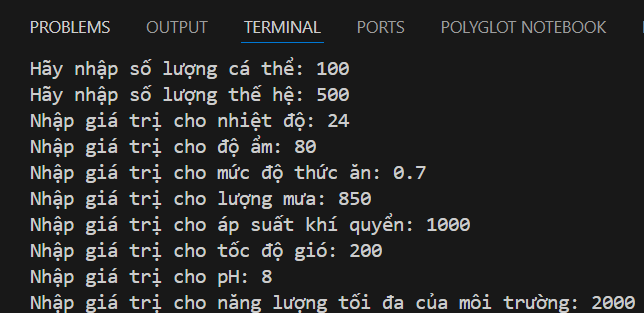
\includegraphics{figures/env_infor.png}
		\caption{Thông tin môi trường. Được nhập từ màn hình Console với thông tin được mô tả ở mục trên}
		\label{fig:env_infor}
	\end{figure}
	
	Với thông số trên, tiến hành đào tạo quần thể gồm 100 cá thể, qua 500 thế hệ, ta có kết quả:
	\begin{figure}[h]
		\centering
		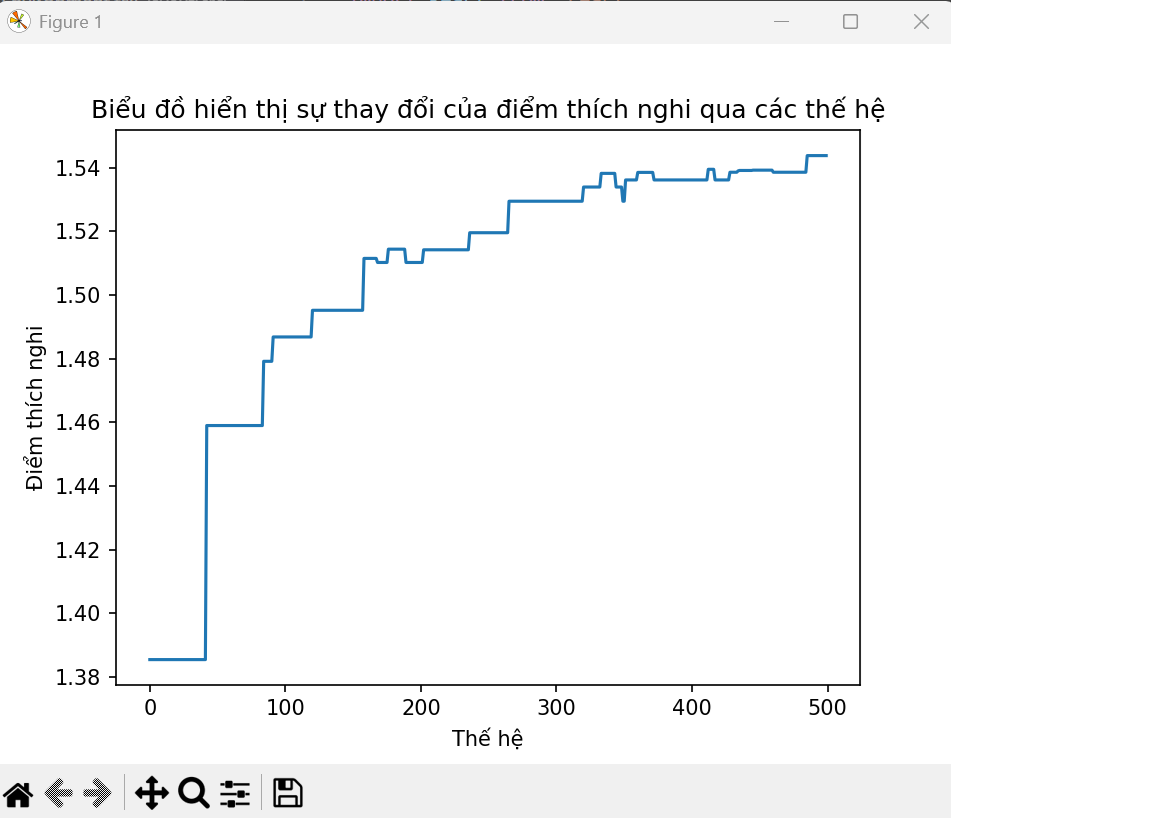
\includegraphics[scale=0.6]{figures/result.png}
		\caption{Biểu đồ ghi nhận giá trị Fitness cao nhất qua các thể hệ. Tuy có những thế hệ mà điểm Fitness tăng rùi lại giảm (do tác động của tính ngẫu nhiên) nhưng xu hướng chung là tăng theo thời gian.}
		\label{fig:result}
	\end{figure}
	
	Thực thi trên mã nguồn, sẽ hiển thị được thêm một số kết quả khác như thông số cài đặt thuật toán, mối quan hệ tổ tiên của một cá thể, ...